\chapter{变分法}\label{ch:variation}

\begin{guidebox}
从两条连接同一对端点的路线开始。你可以比较它们的长度，也可以比较走完全程需要多久。每条路线都算出一个数，这种用整条函数作输入的规则叫泛函。把其中一条路线稍微挪一挪，比较所得数值怎样改变，就进入了变分法。

先用折射练习只有一个待选点的情形，再把这套做法推广到整条曲线。每次算完一阶变分，记得检查两件事。端点是否允许移动？算出的路径能否进一步证明是极小？第三章会用同一方法从作用量求运动方程。
\end{guidebox}

\section{变分思想：从费马原理开始}
两点之间可以画很多条路。先从光在不同介质中传播的时间开始，看看怎样把选择整条路的问题化成可计算的问题。

\subsection{先说清楚比较哪些路径}
可以给每条路线算一个总长度。改变路线时，先检查两端是否仍接在指定地点，途中是否还满足给定条件。

普通函数 $f(z)$ 的自变量是数，泛函（functional）的自变量是一整条函数。例如固定两端的曲线 $y(x)$，其长度为
\[
\mathcal L[y]=\int_a^b\sqrt{1+y'^2}\,\dd x.
\]
不同曲线给出不同长度，即使它们在端点取相同数值。要问哪一条最短，必须先规定\textbf{容许路径}：定义区间、边界值、光滑性、是否允许自交，以及必须满足的约束。不同的容许集合可能产生不同的答案。

本章先讨论标量图形 $y=y(x)$，通常取 $y\in C^2[a,b]$，扰动取满足端点条件的光滑函数；被积函数在路径邻域具有所需的连续偏导数。含尖点、无穷斜率或分段介质的问题，要单独说明分段求解和极限步骤。参数化曲线适用于不能由单个 $y(x)$ 覆盖的情形。

\subsection{费马原理及其适用范围}
光从空气进入另一种介质时，两段传播速度可能不同。即使把路线拉直会缩短距离，也还要比较总用时。费马原理要求小改路径时，传播时间的一阶变化为零。

在静止、各向同性介质的几何光学近似下，设折射率为正函数 $n(\br)$，局部光速为 $c/n$。沿路径的传播时间与光程为
\begin{equation}\label{eq:fermat}
T[\gamma]=\frac1c\int_\gamma n(\br)\,\dd s,\qquad
\mathcal L_{\rm opt}[\gamma]=\int_\gamma n\,\dd s.
\end{equation}
对固定空间端点的邻近容许路径，费马原理给出
\begin{equation}\label{eq:fermat-variation}
\delta T=0\quad\Longleftrightarrow\quad\delta\mathcal L_{\rm opt}=0.
\end{equation}
这里暂把 $\delta$ 理解为“一阶路径变化”；严格定义将在下一节给出。驻值不预先保证全局最短时间，存在多条光线、焦点或反射约束时尤其如此。
\begin{physicsbox}
比较路径是理论中的操作，不是光线预先知道终点。在短波长近似中，邻近光学路径的相位由光程决定；远离驻相区域的贡献容易相消。这个图像说明几何光学与波动光学的联系，但不能用一句“自然总在优化”代替对容许路径和适用极限的规定。
\end{physicsbox}

\subsection{折射定律：先做一个普通极值问题}
固定光源和终点，先假定每种均匀介质内的光线都是直线。此时唯一要选的是过界面的位置，可以直接对该位置求导。

\begin{example}[固定两端的平面折射]
界面为 $y=0$，$A=(0,h_1)$、$B=(d,-h_2)$，$h_1,h_2,d>0$，两侧均匀折射率为 $n_1,n_2>0$。先在各均匀介质中取直线段，令折射点 $P=(\xi,0)$，则
\[
\mathcal L(\xi)=n_1\sqrt{\xi^2+h_1^2}+n_2\sqrt{(d-\xi)^2+h_2^2}.
\]
求导得到
\[
\mathcal L'(\xi)=n_1\frac{\xi}{\sqrt{\xi^2+h_1^2}}
-n_2\frac{d-\xi}{\sqrt{(d-\xi)^2+h_2^2}}.
\]
定义两侧光线与法线的夹角为 $\theta_1,\theta_2$，驻值条件为
\[
\boxed{n_1\sin\theta_1=n_2\sin\theta_2.}
\]
而
\[
\mathcal L''(\xi)=\frac{n_1h_1^2}{(\xi^2+h_1^2)^{3/2}}
+\frac{n_2h_2^2}{((d-\xi)^2+h_2^2)^{3/2}}>0.
\]
因此本例在折射点这一变量上严格凸，驻点确为唯一最小值。并且 $\mathcal L'(0)<0,\mathcal L'(d)>0$，可知它在两端垂足之间。$n_1=n_2$ 时两段接成同一直线，是结果的直接检验。
\end{example}
\begin{figure}[htbp]
\centering
\begin{tikzpicture}[>=Stealth]
\fill[blue!4] (-2.5,0) rectangle (2.7,2.2);
\fill[blue!12] (-2.5,0) rectangle (2.7,-2.2);
\draw[thick] (-2.5,0)--(2.7,0);
\coordinate (A) at (-1.5,2);\coordinate (P) at (0,0);\coordinate (B) at (1,-2);
\draw[very thick,red!70!black] (A)--(P)--(B);
\draw[dashed] (0,-2.3)--(0,2.3);
\draw (0,.65) arc (90:126.869898:.65);
\draw (0,-.65) arc (-90:-63.434949:.65);
\node at (-.45,.8) {$\theta_1$};\node at (.4,-.85) {$\theta_2$};
\fill (A) circle (2pt) node[above]{$A$};\fill (P) circle (2pt) node[below left]{$P$};
\fill (B) circle (2pt) node[below]{$B$};
\node at (2,1) {$n_1=1$};\node at (2,-1) {$n_2=3/\sqrt5$};
\end{tikzpicture}
\caption{按斯涅尔关系选取的折射示例。两角都从同一界面法线测量；图形斜率与标出的折射率相容。}
\label{fig:var-refraction}
\end{figure}

\subsection{从有限个折射点走向一条未知曲线}
若有许多薄层，每层界面的穿过位置都可以调。层数越来越多时，这一串可调的点便用一条连续曲线来描述。

若把连续变化的介质切成许多薄层，未知量变成每个界面的折射点；层数趋于无穷时，未知量成为整个函数。最速降线也有相同结构：取 $y$ 向下、出发点为原点，均匀重力下无摩擦滑动且初速为零，则由第一章能量守恒，$v=\sqrt{2gy}$。在 $y>0$ 的曲线段上，
\begin{equation}\label{eq:brachistochrone-functional}
T[y]=\int_0^{x_B}\frac{\sqrt{1+y'^2}}{\sqrt{2gy}}\,\dd x.
\end{equation}
最短几何长度与最短时间权衡不同。出发点 $y=0$ 使被积函数奇异，因此不能不加说明地把下面的光滑定理直接用于端点；本章稍后将在内部推导，再检查时间积分的可积性。

\section{泛函、一阶变分与欧拉--拉格朗日方程}
让原曲线稍微鼓起一点，看看整条路径的评分怎样变。把变化的一次项写清楚，就能分别得到曲线内部和端点应满足的条件。

\subsection{有限差、变分与时间位移的区别}
把鼓起的形状固定，只用一个小系数控制鼓起的程度。有限差比较两条已经画好的曲线，一阶变分则看这个系数从零开始改变时，评分变得多快。

考虑
\begin{equation}\label{eq:functional}
I[y]=\int_a^b F(x,y,y')\,\dd x,\qquad y(a)=y_A,\quad y(b)=y_B.
\end{equation}
$F$ 称为被积函数；这里的 $x$ 是独立变量，未必是位置，也可以是时间。取一条试探函数 $y$，选定扰动形状 $\eta(a)=\eta(b)=0$，组成路径族
\[
y_\epsilon(x)=y(x)+\epsilon\eta(x).
\]
$\epsilon$ 是标记路径的小参数。严格定义\textbf{一阶变分}为对参数的方向导数：
\begin{equation}\label{eq:var-definition}
\delta I[y;\eta]=\left.\frac{\dd}{\dd\epsilon}I[y_\epsilon]\right|_{\epsilon=0},
\qquad \delta y=\eta,\quad \delta y'=\eta'.
\end{equation}
本章约定 $\delta y$ 表示单位参数的变分方向，不把 $\epsilon$ 重复包含其中。因此有限变化满足
\[
I[y+\epsilon\eta]-I[y]=\epsilon\delta I[y;\eta]
+\tfrac12\epsilon^2\delta^2I[y;\eta]+o(\epsilon^2).
\]
\textbf{驻值}意味着对所有容许方向都有 $\delta I[y;\eta]=0$；并非要求所有邻近曲线都给出完全相等的泛函值。
\begin{figure}[htbp]
\centering
\begin{tikzpicture}[>=Stealth]
\draw[->] (-.3,0)--(5.5,0) node[right]{$x$};\draw[->] (0,-.2)--(0,2.7) node[above]{$y$};
\draw[very thick,blue!70!black,domain=0:5,samples=100] plot (\x,{.6+.2*\x+.25*sin(36*\x)});
\draw[dashed,red!70!black,domain=0:5,samples=100] plot (\x,{.6+.2*\x+.85*sin(36*\x)});
\draw[<->] (2.5,1.35)--(2.5,1.95);
\draw[thin] (2.5,1.95)--(2.5,2.2);
\node[above] at (2.5,2.2) {$\epsilon\eta(x_*)$};
\fill (0,.6) circle (2pt);\fill (5,1.6) circle (2pt);
\draw[dotted] (2.5,0)--(2.5,1.3);\node[below] at (2.5,0) {$x_*$};
\node[blue!70!black] at (4.4,1.15) {$y$};\node[red!70!black] at (3.8,2.3) {$y_\epsilon$};
\end{tikzpicture}
\caption{在同一个独立变量 $x_*$ 处比较两条路径，竖直差为 $\epsilon\eta(x_*)$；两端相同。变分不是沿原路径从 $x_*$ 走到 $x_*+\dd x$ 的真实位移。}
\label{fig:var-neighbor-paths}
\end{figure}

\subsection{从链式法则到边界项}
曲线的高度和斜率都可能影响积分。把斜率变化那一项分部积分后，一项留在端点，另一项和高度变化一起留在积分里。

对参数 $\epsilon$ 求导，并在光滑条件下交换微分与积分：
\[
\delta I=\int_a^b\left(F_y\eta+F_{y'}\eta'\right)\dd x.
\]
其中各偏导沿未扰动路径 $y(x)$ 取值。$y,y'$ 在求偏导时作为独立槽位；之后才代入 $y'=\dd y/\dd x$。关键的一步是分部积分：
\[
\int_a^b F_{y'}\eta'\dd x
=[F_{y'}\eta]_a^b-\int_a^b\frac{\dd F_{y'}}{\dd x}\eta\dd x.
\]
因此完整的一阶变分为
\begin{equation}\label{eq:variation-boundary}
\delta I=[F_{y'}\eta]_a^b+
\int_a^b\left(F_y-\frac{\dd F_{y'}}{\dd x}\right)\eta\dd x.
\end{equation}
先保留边界项，再根据端点条件处理。固定端点给出 $\eta(a)=\eta(b)=0$，从而
\begin{equation}\label{eq:first-variation}
\delta I=\int_a^b\left(F_y-\frac{\dd F_{y'}}{\dd x}\right)\eta\dd x.
\end{equation}
若括号是连续函数且对所有内部光滑紧支扰动积分均为零，\textbf{变分法基本引理}保证括号逐点为零。理由是：若某点处括号为正，则附近仍为正，取支撑在该邻域的非负扰动即可得到正积分，与假设矛盾；负值同理。故驻值路径满足
\begin{equation}\label{eq:euler-lagrange}
\boxed{F_y-\frac{\dd}{\dd x}F_{y'}=0.}
\end{equation}
这就是欧拉--拉格朗日（Euler--Lagrange）方程，是内部驻值的必要条件，还须满足原边界条件及任何约束。

\begin{example}[一个可直接检验的驻值函数]
令独立变量与函数值均为无量纲量，求
\[
I[y]=\int_0^1(y'^2+2xy)\dd x,\qquad y(0)=0,\quad y(1)=1.
\]
有 $F_y=2x,F_{y'}=2y'$，所以 $y''=x$。两次积分得 $y=x^3/6+C_1x+C_2$，端点给出 $C_2=0,C_1=5/6$。对任意固定端点扰动 $h$，精确展开为
\[
I[y+h]-I[y]=\int_0^1\bigl[2y'h'+2xh+h'^2\bigr]\dd x
=\int_0^1h'^2\dd x>0\quad(h\ne0).
\]
中间用 $y''=x$ 及 $h(0)=h(1)=0$ 消去一次项。因此这个驻点还是整个图形容许类中的唯一全局极小，结论比仅解出方程更强。
\end{example}

\subsection{离散化：把路径看成很多个坐标}
先把曲线画成许多小线段。固定两头，只调中间顶点的高度，就能用熟悉的多变量求极值来近似这个问题。

令 $h=(b-a)/N$、$x_k=a+kh$，固定 $y_0,y_N$，用
\begin{equation}\label{eq:discrete-functional}
I_N=\sum_{k=1}^NhF\left(x_k,y_k,\frac{y_k-y_{k-1}}h\right)
\end{equation}
近似积分。内部 $y_k$ 只影响第 $k$ 和 $k+1$ 项，普通偏导数给出
\begin{equation}\label{eq:discrete-el}
\frac{\partial I_N}{\partial y_k}
=hF_y|_k+F_{y'}|_k-F_{y'}|_{k+1}=0.
\end{equation}
除以 $h$，差分形式趋近 $F_y-\dd F_{y'}/\dd x=0$。这解释连续方程与多元极值条件的联系，但不是一般的数值收敛定理；离散驻点是否逼近指定连续解，还依赖正则性、离散格式和解的稳定性。

\subsection{首次积分与多个未知函数}
有些问题在曲线的不同位置遵守同一条局部规则。这种不显含某个变量的结构有时能直接给一个常量，少解一阶微分方程。

沿驻值路径应用乘积法则，有
\[
\frac{\dd}{\dd x}(F-y'F_{y'})
=F_x+y'\left(F_y-\frac{\dd F_{y'}}{\dd x}\right)=F_x.
\]
若 $F$ 不显含 $x$，则有\textbf{贝尔特拉米恒等式}
\begin{equation}\label{eq:beltrami}
F-y'F_{y'}=C.
\end{equation}
这是沿解成立的首次积分，不是任意曲线上的恒等式；也不保证凡满足它的退化解均满足原欧拉--拉格朗日方程，应代回核验。

若 $I$ 依赖多个函数 $y_i(x)$，在无额外约束时各方向独立，故
\begin{equation}\label{eq:el-multi}
F_{y_i}-\frac{\dd}{\dd x}F_{y_i'}=0,\qquad i=1,\ldots,n.
\end{equation}
若 $F$ 不显含某个 $y_i$，则
\begin{equation}\label{eq:cyclic}
F_{y_i'}=\text{常量}.
\end{equation}
第三章会把这解释为循环坐标与守恒动量。若再作 $F\to F+\dd G(x,y)/\dd x$，泛函只改变 $[G]_a^b$；固定端点时它不改变内部方程，但自由端点时边界条件可能改变。

\section{边界条件和约束：容许变分决定答案}
端点钉在墙上与端点沿导轨滑动，是两种不同的题。写完内部方程以后，还要回来看端点或总长度究竟允许怎样变化。

\subsection{自然边界条件}
如果右端可以上下动，就不能直接把右端变分置零。为了让任意允许的小移动都不产生一次变化，必须要求它所乘的系数为零。

若 $a,b$ 固定，而 $y(b)$ 自由，则先取内部扰动得到欧拉--拉格朗日方程，再任取终点扰动，式 \eqref{eq:variation-boundary} 要求
\begin{equation}\label{eq:natural-bc}
F_{y'}(b)=0.
\end{equation}
起点自由时同理；仅自由的端点才有这条条件，不能在固定端点上额外强加它。若泛函另含端点代价 $B(y(b))$，其变分为 $B_y\eta(b)$。与积分产生的 $F_{y'}(b)\eta(b)$ 相加，再令任意的 $\eta(b)$ 的系数为零，便有 $F_{y'}(b)+B_y=0$。
\begin{example}[到一条竖直直线的最短距离]
取 $I=\int_0^L\sqrt{1+y'^2}\dd x$，$y(0)=0$，终点在 $x=L>0$ 上自由滑动。内部方程给出直线 $y=kx$，边界条件给出 $k/\sqrt{1+k^2}=0$，所以 $y=0$。它垂直目标直线；并且所有容许图形长度至少为 $\int_0^L1\dd x=L$，故确实达到全局最短。

内部方程为 $\dd[y'/\sqrt{1+y'^2}]/\dd x=0$，其括号内函数对 $y'$ 严格单调，故 $y'$ 为常数。积分分部的右端项为 $[y'/\sqrt{1+y'^2}]_{x=L}\eta(L)$，端点可竖直滑动意味着 $\eta(L)$ 任意，因此斜率必须为零。
\end{example}

\subsection{移动端点与横截条件的推导}
端点沿斜线移动时，横坐标和纵坐标会一起改变。先把允许的移动方向写出来，再看边界项沿这个方向的分量是否为零。

现在令终点横坐标也可变，$b_\epsilon=b+\epsilon\Delta b$，终点总纵向变化为 $\Delta y_B$。若 $y_\epsilon(x)=y(x)+\epsilon\eta(x)$，则
\[
y_\epsilon(b_\epsilon)=y(b)+\epsilon[\eta(b)+y'(b)\Delta b]+O(\epsilon^2),
\]
故 $\eta(b)=\Delta y_B-y'(b)\Delta b$。积分上限移动还产生 $F(b)\Delta b$，于是内部方程满足后，终点贡献为
\begin{equation}\label{eq:var-transversality}
\delta I\big|_B=F_{y'}\Delta y_B+(F-y'F_{y'})\Delta b.
\end{equation}
若端点沿 $y_B=\psi(b)$ 移动，$\Delta y_B=\psi'(b)\Delta b$，由 $\Delta b$ 的任意性得到\textbf{横截条件}
\[
\boxed{F+(\psi'-y')F_{y'}=0\quad\text{在终点成立}.}
\]
对长度泛函，化为 $1+y'\psi'=0$，即两切线正交。目标竖直线应采用前面的固定 $b$ 情形，不应把无穷大的 $\psi'$ 硬代入这个公式。
\begin{figure}[htbp]
\centering
\begin{tikzpicture}[>=Stealth]
\draw[thick,gray] (-.5,0)--(4,2.25) node[right]{目标直线};
\coordinate (B) at (2,1.25);\coordinate (A) at (3,-.75);
\draw[very thick,blue!70!black] (A)--(B);
\draw[->,thick,red!70!black] (B)--(3,1.75) node[above]{$\Delta\br_B$};
\fill (A) circle (2pt) node[below]{$A$};\fill (B) circle (2pt) node[above left]{$B$};
\draw (2.16,.93)--(2.48,1.09)--(2.32,1.41);
\end{tikzpicture}
\caption{移动端点的容许位移沿目标线。最短连接段垂直目标线，正交条件来自终点边界项，而非内部微分方程。}
\label{fig:var-free-end}
\end{figure}

\subsection{积分约束与乘子的条件}
规定绳长后，可以改一小段的形状，但其他段可能需要同时调整，才能保持总长。用一个乘子把总长条件和原目标放到同一个变分式中。

设还要求 $J[y]=\int_a^bG(x,y,y')\dd x=\ell$。在约束正则，即一阶线性泛函 $\delta J$ 不恒为零的条件下，受约束驻点满足存在\textbf{常数} $\lambda$ 使
\begin{equation}\label{eq:lagrange-multiplier}
\delta(I-\lambda J)=0,
\end{equation}
也就是对 $\widetilde F=F-\lambda G$ 求
\begin{equation}\label{eq:constrained-el}
\widetilde F_y-\frac{\dd}{\dd x}\widetilde F_{y'}=0.
\end{equation}
乘子与积分上限无关，由边界值和积分约束共同确定。取固定端点扰动 $\zeta$ 满足 $\delta J[\zeta]\ne0$。对任意满足 $\delta J[\eta]=0$ 的固定端点扰动，用隐函数定理选择 $u(\epsilon)$，使 $J[y+\epsilon\eta+u(\epsilon)\zeta]=\ell$。对约束求导得 $u'(0)=0$，所以受约束驻点满足 $\delta I[\eta]=0$。对一般扰动 $\eta$，减去 $\zeta\,\delta J[\eta]/\delta J[\zeta]$ 就得到这样的核方向。由线性性，$\delta I=\lambda\delta J$，其中 $\lambda=\delta I[\zeta]/\delta J[\zeta]$。若 $\delta J$ 处处为零，这个常规推理失效，需分析异常约束，不能直接套用归一化乘子形式。

点态约束 $g(x,y_1,\ldots,y_n)=0$ 则在每个 $x$ 都施加条件，通常引入函数乘子 $\lambda(x)$。积分约束的常数乘子和点态约束的函数乘子不要混淆。第三章还会说明：对非完整速度约束，简单把约束加入作用量未必给出物理运动。

\begin{example}[圆弧面积问题：限制图形类后再求解]
固定端点 $(0,0),(d,0)$，要求 $y(x)\ge0$ 且弧长为 $\ell$。本例先限制为光滑图形，并取 $d<\ell<\pi d/2$。最大化面积 $A=\int_0^dy\dd x$。令
\[
\widetilde F=y-\lambda\sqrt{1+y'^2},
\qquad
1+\lambda\frac{y''}{(1+y'^2)^{3/2}}=0.
\]
曲率为常数，取上凸圆弧对应 $\lambda=R>0$。由对称性，圆心横坐标为 $d/2$。用半圆心角 $0<\alpha<\pi/2$ 表示，
\[
d=2R\sin\alpha,\qquad \ell=2R\alpha,\qquad
\frac\ell d=\frac\alpha{\sin\alpha},
\]
\[
y_*(x)=\sqrt{R^2-(x-d/2)^2}-R\cos\alpha.
\]
上述比例在此范围单调，端点与长度唯一确定 $R,\alpha$。还可以证明极大性：$-R\sqrt{1+p^2}$ 对斜率 $p$ 严格凹，而 $y$ 项线性，故对任意同端点图形
\[
(A-R\mathcal L)[y]-(A-R\mathcal L)[y_*]
\le\delta(A-R\mathcal L)[y_*;y-y_*]=0.
\]
若弧长相同，便有 $A[y]\le A[y_*]$，等号只对应同一图形。

不能把这个图形证明无条件用于任意大弧长：$\ell\to\pi d/2$ 时圆弧趋于半圆，端点斜率发散；再大的圆弧会有回折，不能由一个光滑 $y(x)$ 表示。闭合曲线等周定理需要参数化曲线的容许类，本例没有假装已证明它的全部版本。
\end{example}

\section{二阶变分：驻值为什么不一定是极小？}
一个数的导数为零可能对应谷底、山顶或更平的地方。对整条曲线也要做第二步检查，看看往各个允许方向稍作改变时，原量是增还是减。

\subsection{二次型、必要条件与充分条件}
同一条曲线可以有很多种鼓起方式。二阶变分要检查的是这些方式各自引起的二次变化，其中只要有一个方向使它减小，就排除了极小。

固定端点时，对同一族 $y+\epsilon\eta$ 再求一次参数导数，定义
\[
\delta^2 I[y;\eta]=\left.\frac{\dd^2}{\dd\epsilon^2}I[y+\epsilon\eta]\right|_0.
\]
注意在泰勒展开中它前面有 $1/2$，这只是约定，不影响符号。直接求导两次：
\begin{align}\label{eq:second-variation}
\delta^2 I
&=\int_a^b(F_{yy}\eta^2+2F_{yy'}\eta\eta'+F_{y'y'}\eta'^2)\dd x\nonumber\\
&=\int_a^b\left(P\eta'^2+Q\eta^2\right)\dd x,\qquad
P=F_{y'y'},\quad Q=F_{yy}-\frac{\dd F_{yy'}}{\dd x}.
\end{align}
第二步对 $2F_{yy'}\eta\eta'=F_{yy'}(\eta^2)'$ 分部积分，端点项因 $\eta=0$ 消失。各系数沿待检验的驻值路径取值。

局部极小要求 $\delta^2I\ge0$ 对所有容许方向成立，这是必要条件；若存在正、负两种方向，则为鞍点。对正则标量问题，局部极小还必须满足勒让德条件 $F_{y'y'}\ge0$。严格的 $F_{y'y'}>0$ 常作为加强条件，但它\textbf{单独并不保证极小}，因为 $Q\eta^2$ 可能贡献负值。

在无限维函数空间里，也不能不说明拓扑和余项控制，就将“每个方向二阶导数均正”直接当作统一邻域内的充分条件。一个实用的充分条件是：$F$ 在候选路径附近足够光滑，二次型有统一正下界
\[
\delta^2I[y;\eta]\ge c\int_a^b\eta'^2\dd x,\qquad c>0,
\]
且泰勒余项相对于该范数可一致控制。例如连续系数满足 $P\ge p_0>0,Q\ge0$ 时，配合固定端点的庞加莱不等式即可得到所需估计，因而在足够小的 $C^1$ 邻域内有严格弱极小。这里“弱”指函数值和一阶导数均接近，不是说极小结论不严格。

\begin{example}[直线不仅驻值，而且全局最短]
对 $F=\sqrt{1+y'^2}$，有 $P=(1+y'^2)^{-3/2}>0,Q=0$。固定两端的驻值路径为直线，因此二阶变分为正。还可不依赖局部判据：对任意参数化路径，$\int|\dd\br|\ge|\br_B-\br_A|$，等号对应同向直线段。这个三角不等式给出全局最短，且说明同一直线若往返折返，虽仍落在一条直线上，却不达到等号。
\end{example}

\subsection{作用量随时间区间改变性质的例子}
谐振子的零路径在短区间和长区间都能满足运动方程。不过端点相隔越远，中间可容纳的扰动越多，作用量的极小性可能随之改变。

取谐振子作用量
\[
S[q]=\frac m2\int_0^T(\dot q^2-\omega^2q^2)\dd t,
\qquad q(0)=q(T)=0,\quad m,\omega>0.
\]
$q_*=0$ 对所有 $T$ 都是驻值路径。对固定端点扰动 $\eta$，
\[
\delta^2S=m\int_0^T(\dot\eta^2-\omega^2\eta^2)\dd t.
\]
取 $\eta=A\sin(n\pi t/T)$，利用正弦与余弦平方的积分均为 $T/2$，得
\begin{equation}\label{eq:var-osc-mode}
\delta^2S=\frac{mA^2T}{2}\left[\left(\frac{n\pi}{T}\right)^2-\omega^2\right].
\end{equation}
若 $T<\pi/\omega$，固定端点的庞加莱不等式
$\int\dot\eta^2\dd t\ge(\pi/T)^2\int\eta^2\dd t$
保证所有非零方向均为正；本例是精确二次泛函，所以 $q=0$ 还是全局严格极小。若 $T=\pi/\omega$，$\eta=A\sin\omega t$ 给出零二阶变分，而且这些路径的作用量确实全都为零，极小不严格。若 $T>\pi/\omega$，$n=1$ 给负方向，足够大的 $n$ 给正方向，故是鞍点。
\begin{physicsbox}
“最小作用量”是传统名称。即使 $F_{\dot q\dot q}=m>0$，谐振子在较长时间区间的作用量仍有负变分方向。作用量极小性也不等同于动力学稳定性：谐振子的轨道稳定，并不意味着任意两时刻之间的作用量都是最小值。
\end{physicsbox}
\begin{figure}[htbp]
\centering
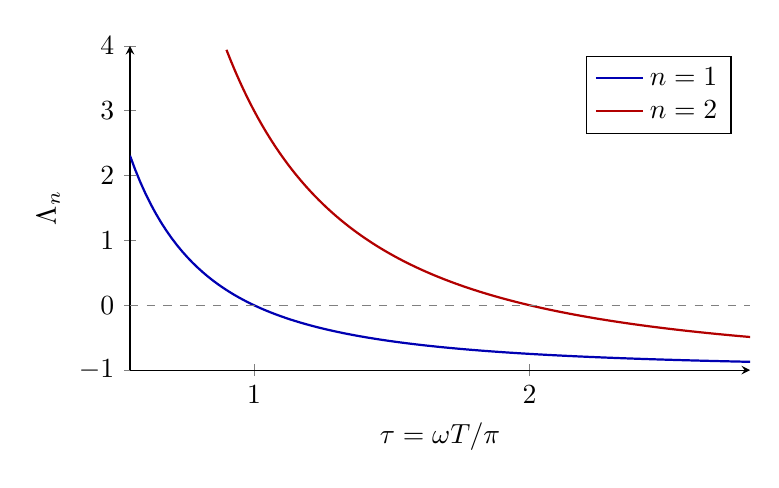
\begin{tikzpicture}
\begin{axis}[width=.78\textwidth,height=5.7cm,axis lines=left,
 xlabel={$\tau=\omega T/\pi$},ylabel={$\Lambda_n$},xmin=.55,xmax=2.8,ymin=-1,ymax=4,
 xtick={1,2},ytick={-1,0,1,2,3,4},legend style={at={(.97,.97)},anchor=north east}]
\addplot[thick,blue!70!black,domain=.55:2.8,samples=120] {1/x^2-1};
\addplot[thick,red!70!black,domain=.9:2.8,samples=120] {4/x^2-1};
\addplot[dashed,gray,domain=.55:2.8] {0};
\legend{$n=1$,$n=2$}
\end{axis}
\end{tikzpicture}
\caption{无量纲二阶变分系数 $\Lambda_n=n^2/\tau^2-1$。第一个模在 $T=\pi/\omega$ 变号；一个负模已足以否定极小性。图线由式 \eqref{eq:var-osc-mode} 直接绘出。}
\label{fig:var-second-sign}
\end{figure}

\subsection{进一步探索：雅可比方程与共轭点}
有时存在一个小扰动，从起点出发后恰好又在某个时刻回到零。找出这个时刻，有助于判断原路径的极小性质何时可能改变。

对二次型 $\mathcal Q[\eta]=\int(P\eta'^2+Q\eta^2)\dd x$ 作变分，内部驻值条件为
\begin{equation}\label{eq:jacobi}
-\frac{\dd}{\dd x}(P\eta')+Q\eta=0.
\end{equation}
它是\textbf{零模方程}；若要在 $\int\eta^2\dd x=1$ 下最小化该二次型，则右边是 $\lambda\eta$，不能漏掉归一化乘子。总存在零解，讨论共轭点时寻找的是非平凡解。

在 $P>0$ 且系数正则的标量问题中，固定起点 $a$，若存在非平凡解满足 $\eta(a)=\eta(c)=0$，则称 $c>a$ 与 $a$ 共轭。它不是要求区间内完全不存在非零解，而是要求不存在具有指定两个零点的解。加强勒让德条件与区间 $(a,b]$ 上无共轭点相结合，给出通常的固定端点严格弱极小判据；证明涉及二次型分解，作为进阶阅读，不用它替代前面已给出的直接检查。

谐振子中 $P=m,Q=-m\omega^2$，雅可比方程是 $\ddot\eta+\omega^2\eta=0$，起点为零的非平凡解正比于 $\sin\omega t$，首个共轭时刻正是 $\pi/\omega$，与上面的模态计算一致。学习这个拓展需要二阶线性常微分方程和边值问题。

\section{几何与力学中的变分问题}
找最短路、算绳子的形状和比较下滑时间，分别要最小化或取驻值的是长度、势能和时间。先写明每题比较什么，再套用变分步骤。

\subsection{平面最短路径与曲面测地线}
平面上能直接连直线，球面上则只能沿表面走。即使一段大圆弧处处符合测地线方程，也应比较同一对端点间另一侧的弧长。

长度泛函的被积函数不显含 $y$，由式 \eqref{eq:cyclic} 得 $y'/\sqrt{1+y'^2}=C$，所以 $y'$ 为常数，端点确定直线。

在曲面上，使用局部坐标 $q^1,q^2$，定义正定度规
\[
\dd s^2=g_{ij}(q)\dd q^i\dd q^j,
\]
重复指标求和，$g_{ij}=g_{ji}$，逆矩阵为 $g^{ij}$。用任意正则参数 $u$ 表示曲线，令
\[
N=\sqrt{g_{ij}q'^iq'^j},\qquad \mathcal L=\int N\dd u,
\]
此处撇号表示 $\dd/\dd u$，$u$ 不必是物理时间。先求偏导：
\[
N_{q'^k}=\frac{g_{kj}q'^j}{N},\qquad
N_{q^k}=\frac{\partial_kg_{ij}q'^iq'^j}{2N}.
\]
将它们代入欧拉--拉格朗日方程，乘以 $N$ 并展开：
\[
g_{kj}q''^j+\partial_i g_{kj}q'^iq'^j
-\frac12\partial_kg_{ij}q'^iq'^j
=\frac{N'}N g_{kj}q'^j.
\]
把二次速度项对称化，乘以 $g^{mk}$，得到
\[
q''^m+\Gamma^m_{ij}q'^iq'^j=\frac{N'}Nq'^m,
\]
\begin{equation}\label{eq:christoffel}
\Gamma^m_{ij}=\frac12g^{mk}(\partial_i g_{kj}+\partial_j g_{ki}-\partial_k g_{ij}).
\end{equation}
若在导出方程后选择弧长 $s$ 或其仿射变换为参数，$N$ 为常数，右侧消失：
\begin{equation}\label{eq:geodesic}
\boxed{\frac{\dd^2q^m}{\dd s^2}+\Gamma^m_{ij}\frac{\dd q^i}{\dd s}\frac{\dd q^j}{\dd s}=0.}
\end{equation}
不能先把 $N=1$ 代入被积函数再变分，那样会错误地把长度泛函变成常数。测地线是弧长驻值的曲线，只在足够短、未跨过相应共轭点的弧段上保证局部最短，未必全局最短。

\begin{example}[球面：大圆长弧为何不是最短？]
半径为 $R$ 的球面，取 $q^1=\theta,q^2=\varphi$，有
\[
g_{\theta\theta}=R^2,\quad g_{\varphi\varphi}=R^2\sin^2\theta.
\]
唯一非零的度规偏导是 $\partial_\theta g_{\varphi\varphi}=2R^2\sin\theta\cos\theta$。因此
\[
\Gamma^\theta_{\varphi\varphi}=-\sin\theta\cos\theta,\qquad
\Gamma^\varphi_{\theta\varphi}=\Gamma^\varphi_{\varphi\theta}=\cot\theta,
\]
\[
\theta''-\sin\theta\cos\theta\,\varphi'^2=0,\qquad
\varphi''+2\cot\theta\,\theta'\varphi'=0,
\]
撇号现表示对弧长求导。赤道解为 $\theta=\pi/2,\varphi=\varphi_0\pm s/R$；系数须满足单位速率条件，不能任取。球面对称性及初值唯一性说明一般正则测地线是大圆的一段。

两个非对跖点间存在同一大圆上的短弧和长弧，长度分别为 $R\beta$ 与 $R(2\pi-\beta)$，$0<\beta<\pi$。两者都满足测地线方程，只有短弧是全局最短。对跖点间则有无穷多等长的大圆半圆，最短路径不唯一。球坐标的极点奇异需换坐标，不是曲面本身有奇点。
\end{example}
\begin{figure}[htbp]
\centering
\begin{tikzpicture}[>=Stealth]
\draw[very thick,gray!65] (0,0) circle (1.8);
\draw[very thick,blue!70!black] (1.8,0) arc (0:110:1.8);
\fill (1.8,0) circle (2pt) node[right]{$A$};
\fill ({1.8*cos(110)},{1.8*sin(110)}) circle (2pt) node[above]{$B$};
\draw[dashed] (0,0)--(1.8,0);\draw[dashed] (0,0)--({1.8*cos(110)},{1.8*sin(110)});
\draw (.6,0) arc (0:110:.6);\node at (.6,.6) {$\beta$};
\node[blue!70!black] at (1.6,1.6) {短弧};\node[gray!65] at (-1.8,-1.5) {长弧};
\end{tikzpicture}
\caption{在过球心的大圆平面中观察两端点。短、长两弧均是球面测地线；满足驻值方程不等于在所有连接路径中长度最小。}
\label{fig:var-great-circle}
\end{figure}

\subsection{悬链线：坐标方向、长度约束与张力}
均匀绳子下垂时，靠近支点的张力要托住更多绳段。由于载荷按绳的弧长分布，坡越陡，每单位水平距离要托住的绳子也越多。

\begin{example}[均匀柔绳的平衡形状]
柔绳线密度为 $\rho_\ell$，两端固定，绳长为 $\ell$，不可伸长，忽略弯曲刚度，均匀重力竖直向下。本例取 $y$ 向上，故势能应为
\[
V[y]=\rho_\ell g\int y\dd s
=\rho_\ell g\int y\sqrt{1+y'^2}\dd x,
\]
不能写成与向上坐标相反的负号。固定长度 $\mathcal L=\int\sqrt{1+y'^2}\dd x=\ell$，将常数 $\rho_\ell g$ 提出，并用长度量纲的乘子 $\lambda$，得到
\[
\widetilde F=(y-\lambda)\sqrt{1+y'^2}.
\]
由于不显含 $x$，式 \eqref{eq:beltrami} 给出
\[
\frac{y-\lambda}{\sqrt{1+y'^2}}=a.
\]
选择实际下垂、张力为正的分支 $a>0$。由平方关系
\[
y'^2=\frac{(y-\lambda)^2-a^2}{a^2}
\]
分离变量。在最低点右侧取正斜率，左侧取负斜率，两支合起来为
\begin{equation}\label{eq:var-catenary}
y=\lambda+a\cosh\frac{x-x_0}{a}
=y_{\min}+a\left[\cosh\frac{x-x_0}{a}-1\right],
\qquad y_{\min}=\lambda+a.
\end{equation}
$x_0$、$a$ 和高度常数须由两端位置及绳长确定，不能只通过“吸收常数”忽略物理支点高度。

对等高支点 $(-d,H),(d,H)$，有 $x_0=0$，
\[
\ell=\int_{-d}^d\cosh(x/a)\dd x=2a\sinh(d/a),\qquad
H-y_{\min}=a[\cosh(d/a)-1].
\]
当 $\ell>2d$，长度方程给出唯一 $a>0$；$\ell\downarrow2d$ 时 $a\to\infty$，绳近乎拉直，有限重量下张力趋大。若 $\ell<2d$，不可伸长绳根本无法连接支点。

从第一章受力分析独立核验：设水平张力分量 $H_T$ 恒定，以最低点为弧长原点，带符号弧长为
\[s=a\sinh(x/a).\]
竖直张力分量为 $\rho_\ell gs$，切线斜率为
\[
y'=\frac{\rho_\ell gs}{H_T}=\sinh(x/a)
\quad\Longrightarrow\quad H_T=\rho_\ell ga.
\]
这既确认了坐标符号，也说明 $a$ 的力学意义。变分方程给出平衡候选，实际悬挂支取正张力；这里没有仅凭一阶变分就宣称所有可能曲线类中的全局唯一稳定性。
\end{example}
\begin{figure}[htbp]
\centering
\begin{tikzpicture}[>=Stealth]
\draw[->] (-2.6,0)--(2.7,0) node[right]{$x$};\draw[->] (0,-.2)--(0,3) node[above]{$y$};
\draw[very thick,blue!70!black,domain=-2:2,samples=120] plot (\x,{1.5*(cosh(\x/1.5)-1)+.4});
\fill (-2,{1.5*(cosh(2/1.5)-1)+.4}) circle (2pt) node[above left]{$(-d,H)$};
\fill (2,{1.5*(cosh(2/1.5)-1)+.4}) circle (2pt) node[above right]{$(d,H)$};
\fill (0,.4) circle (2pt) node[below right]{$y_{\min}$};
\draw[->,thick,red!70!black] (1.25,1)--(1.25,.25) node[right]{$\bg$};
\end{tikzpicture}
\caption{由解析双曲余弦函数绘制的下垂绳。$y$ 向上而重力向下；绳长是沿弧线的积分，不能误用水平跨度。}
\label{fig:var-catenary}
\end{figure}
\begin{physicsbox}
均匀绳的重量按\emph{弧长}均匀分布，产生悬链线；若悬索负载主要按\emph{水平长度}均匀分布，受力方程不同，可得到抛物线。曲线看起来接近不代表模型相同。悬链线在 $|x-x_0|\ll a$ 时也有局部展开 $y\simeq y_{\min}+(x-x_0)^2/(2a)$。
\end{physicsbox}

\subsection{最速降线：解、端点与时间验证}
陡一点的路线能更早获得速度，却也可能绕得更远。最速降线正是比较沿途速度与路程这两方面后得到的路径。

本例重新取 $y$ 向下。内部 $y>0$ 时，令
\[
F=\frac{\sqrt{1+y'^2}}{\sqrt{2gy}},
\qquad F-y'F_{y'}=\frac1{\sqrt{2gy}\sqrt{1+y'^2}}=C>0.
\]
定义 $a=1/(4gC^2)>0$，得到
\begin{equation}\label{eq:brachistochrone-ode}
y'^2=\frac{2a-y}{y}.
\end{equation}
在首拱令 $y=a(1-\cos\theta)$，并令 $\theta$ 随 $x$ 增大。式 \eqref{eq:brachistochrone-ode} 给出 $y'^2=\cot^2(\theta/2)$。下行与回升段分别取 $y'$ 的正根和负根，两段合写为 $y'=\cot(\theta/2)$。由链式法则
\[
\frac{\dd x}{\dd\theta}
=\frac{a\sin\theta}{\cot(\theta/2)}
=a(1-\cos\theta),
\]
在 $\theta=\pi$ 处按连续极限取值。用 $x(0)=0$ 积分，得
\begin{equation}\label{eq:cycloid}
\boxed{x=a(\theta-\sin\theta),\qquad y=a(1-\cos\theta).}
\end{equation}
当 $0<\theta<\pi$，$x_\theta=a(1-\cos\theta)>0$、$y_\theta=a\sin\theta>0$，曲线下行；$\pi<\theta<2\pi$ 时 $x$ 仍增大而 $y$ 减小，曲线回升。故分离变量写 $\dd x=\sqrt{y/(2a-y)}\dd y$ 只适用于前一支，不能用正根覆盖整条摆线。

由端点 $B=(X,Y)$，$X,Y>0$，要求
\[
\frac XY=\frac{\theta_B-\sin\theta_B}{1-\cos\theta_B},\qquad
 a=\frac Y{1-\cos\theta_B}.
\]
设 $u=\theta_B/2$。上述比值对 $\theta_B$ 的导数分子为 $2(1-\cos\theta_B)-\theta_B\sin\theta_B=4\sin u(\sin u-u\cos u)$，分母为 $(1-\cos\theta_B)^2$。由于 $(\sin u-u\cos u)'=u\sin u>0$，且该括号在 $u=0$ 为零，导数在首拱为正。比值两端的极限分别为零与正无穷，故正端点唯一确定首拱参数解；若 $X/Y<\pi/2$，终点在下行段，若 $X/Y>\pi/2$，最速降线候选先降到终点以下再回升，不能始终描述成“先陡后平”。

直接计算弧元和速度：
\[
\frac{\dd s}{\dd\theta}=2a\sin(\theta/2),\qquad
v=\sqrt{2gy}=2\sqrt{ga}\sin(\theta/2),
\]
于是
\begin{equation}\label{eq:var-brach-time}
\dd t=\sqrt{a/g}\dd\theta,\qquad T_B=\theta_B\sqrt{a/g}.
\end{equation}
尽管起点速度为零、切线竖直，二者的零因子相消后时间积分有限。这是对起点奇性的检查；曲线不是在端点具有有限导数的 $C^2$ 图形，前面的正则推导仅用于内部。

\begin{example}[同一终点下与直线比较]
取教学参数 $X=Y=1\,\mathrm m$、$g=9.8\,\mathrm{m/s^2}$。端点方程数值求得 $\theta_B\simeq2.4120$、$a\simeq0.5729\,\mathrm m$，故 $T_B\simeq0.583\,\mathrm s$。直线长为 $D=\sqrt{X^2+Y^2}$，沿线的恒定加速度为 $gY/D$，所以
\[
T_{\rm line}=\sqrt{\frac{2D}{gY/D}}
=\sqrt{\frac{2(X^2+Y^2)}{gY}}\simeq0.639\,\mathrm s.
\]
两条路径使用相同起点、终点、初速及重力模型，比较才有意义。该数值不是实际实验测量。

直线的弧长为 $\sqrt{X^2+Y^2}$，以沿线弧长 $s$ 参数化时 $y=Ys/\sqrt{X^2+Y^2}$，从静止出发有 $v=\sqrt{2gy}$。积分 $\int\dd s/v$ 得 $t_{\rm line}=\sqrt{2(X^2+Y^2)/(gY)}$，再与摆线时间 $\sqrt{a/g}\,\theta_B$ 比较。
\end{example}
\begin{figure}[htbp]
\centering
\begin{tikzpicture}[>=Stealth,x=2.7cm,y=-1.8cm]
\draw[->] (0,0)--(2.15,0) node[right]{$x/a$};\draw[->] (0,0)--(0,2.25) node[below]{$y/a$};
\draw[dashed,gray] (0,0)--({2.4-sin(2.4 r)},{1-cos(2.4 r)});
\draw[very thick,blue!70!black,domain=0:2.4,samples=150]
 plot ({\x-sin(\x r)},{1-cos(\x r)});
\fill (0,0) circle (1pt) node[above left]{$A$};
\fill ({2.4-sin(2.4 r)},{1-cos(2.4 r)}) circle (1pt) node[right]{$B$};
\node[gray] at (.9,.6) {直线};\node[blue!70!black] at (.6,1.5) {摆线};
\end{tikzpicture}
\caption{参数为 $0\le\theta\le2.4$ 的精确摆线及同端点直线。$y$ 轴向下，与能量关系 $v^2=2gy$ 的约定一致。}
\label{fig:var-brachistochrone}
\end{figure}

\paragraph{何时已证明“最速”，而非只求到驻值？}
对下行段 $0<\theta_B<\pi$，可在单调深度的路径类中以 $y$ 为自变量，写 $x=x(y)$。时间泛函变为
\[
T[x]=\int_0^Y f(y,w)\dd y,\quad w=\frac{\dd x}{\dd y},\qquad
f(y,w)=\frac{\sqrt{1+w^2}}{\sqrt{2gy}}.
\]
$f_{ww}>0$，且摆线解上 $f_w$ 是常数。因此凸性给出
\[
T[x]-T[x_*]\ge\int_0^Y f_w(y,x_*')(x'-x_*')\dd y
=C_x[x-x_*]_0^Y=0.
\]
在端点极限可积、同端点且有限时间的这类图形中，摆线达到严格最小。这里利用了一个比欧拉--拉格朗日方程更强的论证。对于允许深度回升的更大曲线类，或 $\theta_B>\pi$ 的情形，本段单调深度证明不适用；完整最速降线理论需另作参数化比较，本章不将其冒充为已证明的结论。

\subsection{作用量初步：从变分返回牛顿方程}\label{sec:action-first}
比较的是同一时间区间上连接同一对端点的路径。先给每条路径算动能减势能的时间积分，再检查小改路径时这个积分怎样变化。

\begin{example}[固定时间端点的一维保守粒子]
取质量恒定、势能 $V(q)$ 光滑的粒子，定义
\[
L(q,\dot q)=\tfrac12m\dot q^2-V(q),\qquad
S[q]=\int_{t_1}^{t_2}L\dd t.
\]
固定 $t_1,t_2$ 及两端位置，取 $q_\epsilon=q+\epsilon\eta$、$\eta(t_1)=\eta(t_2)=0$。逐项变分并分部积分：
\[
\delta S=\int_{t_1}^{t_2}(m\dot q\dot\eta-V'(q)\eta)\dd t
=[m\dot q\eta]_{t_1}^{t_2}-\int_{t_1}^{t_2}(m\ddot q+V')\eta\dd t.
\]
由扰动的任意性得 $m\ddot q=-V'(q)$。在此模型与边界条件下，牛顿方程与哈密顿驻作用量条件相互对应；不是对所有力学系统、非完整约束或耗散系统都无条件等价。
\end{example}
作用量的量纲是能量乘时间；它不是能量，也不要求沿真实轨道每时刻最小。给定 $L$ 是指定动力学模型，$\delta S=0$ 才是求其运动的规则。第\ref{sec:ham-principle}节将用独立广义坐标写出相应的多自由度方程。

\section{进一步探索：从几何光学到受约束优化}
同样的思想还能处理光线在连续介质中弯曲、整根弦一起运动，以及怎样安排随时间变化的控制量。

本节各项是拓展应用，不要求初学者掌握所有推导。它们分别展示多分量路径、空间场和动力学约束；不能把任意优化问题都笼统称为同一个物理原理。
\subsection{梯度折射率中的光线方程}
折射率连续变化时，可以把介质想成许多性质略有差别的薄层。光线的方向在每一小段上微调，整体看便是弯曲的。

设 $\br(u)$ 为正则路径，$I=\int n(\br)|\br'|\dd u$。对各坐标分量取偏导，
\[
\frac{\partial F}{\partial r_i'}=n\frac{r_i'}{|\br'|},\qquad
\frac{\partial F}{\partial r_i}=|\br'|\partial_i n.
\]
欧拉--拉格朗日方程给出
\[
\frac{\dd}{\dd u}\left(n\frac{\br'}{|\br'|}\right)=|\br'|\nabla n.
\]
导出后再取弧长 $s$ 为参数，得到
\begin{equation}\label{eq:ray-equation}
\boxed{\frac{\dd}{\dd s}\left(n\frac{\dd\br}{\dd s}\right)=\nabla n.}
\end{equation}
令 $\be_t=\dd\br/\dd s$，用 $\dd n/\dd s=\be_t\cdot\nabla n$ 分离出
\[
n\frac{\dd\be_t}{\dd s}=\nabla n-\be_t(\be_t\cdot\nabla n).
\]
只有折射率梯度的横向部分使光线弯曲；沿切向的梯度改变 $n\be_t$ 的大小。均匀介质中方向不变。

\begin{example}[近轴梯度折射率模型]
理想折射率在轴附近满足 $n^2(x,y)=n_0^2[1-\alpha^2(x^2+y^2)]$，$\alpha$ 的量纲为逆长度。仅在 $\alpha r\ll1$ 且 $|\dd x/\dd z|,|\dd y/\dd z|\ll1$ 的近轴范围使用此模型，则 $n\simeq n_0(1-\alpha^2r^2/2)$、$\dd s\simeq\dd z$。保留线性横向项，
\[
n_0\frac{\dd^2x}{\dd z^2}\simeq\partial_xn=-n_0\alpha^2x,
\qquad \frac{\dd^2y}{\dd z^2}\simeq-\alpha^2y.
\]
给定 $x(0)=x_0,x'(0)=\beta_0$，
\[
x(z)=x_0\cos\alpha z+\frac{\beta_0}{\alpha}\sin\alpha z.
\]
空间周期为 $2\pi/\alpha$，不是时间周期；$\alpha\to0$ 恢复直线 $x=x_0+\beta_0z$。对一般不同横向相位，三维光线不必落在一张平面中，不能一概称为平面正弦线。模型只处理给定光线的几何传播，不据此计算完整波导模或通信色散性能。
\end{example}
\begin{figure}[htbp]
\centering
\begin{tikzpicture}[>=Stealth]
\fill[blue!5] (0,-1) rectangle (6.6,1);
\draw[dashed,gray] (0,0)--(7,0) node[right]{$z$};
\draw[thick,red!70!black,domain=0:6.6,samples=150] plot (\x,{.65*cos(\x r)});
\draw[<->] (0,1.3)--(6.283185,1.3) node[midway,above]{$2\pi/\alpha$};
\node[left] at (0,.65) {$x_0$};
\end{tikzpicture}
\caption{近轴平面光线的解析示意，$\beta_0=0$，横轴按 $\alpha z$ 缩放。背景仅标示可用的轴附近区域，不表示已指定实际光纤的包层结构。}
\label{fig:var-grin}
\end{figure}

\begin{example}[折射率为 $n(y)=y_0/y$ 的理想介质]
限定 $y>0,y_0>0$，局部用 $x=x(y)$ 表示光线。$F=y_0\sqrt{1+x'^2}/y$ 不显含 $x$，故
\[
\frac{y_0x'}{y\sqrt{1+x'^2}}=C,\qquad k=C/y_0.
\]
若 $k\ne0$，在 $|ky|<1$ 的单调 $y$ 分支上，保留 $k$ 的符号得
\[
x'=\frac{ky}{\sqrt{1-k^2y^2}},\qquad
x-x_0=-\frac1k\sqrt{1-k^2y^2}.
\]
因此 $(x-x_0)^2+y^2=1/k^2$。完整光线可用参数拼接为上半平面的圆弧；另一侧分支需改变参数图，不是关于 $x$ 轴反射到禁用的 $y<0$ 区域。若 $C=0$，还存在 $x=\mathrm{const}$ 的竖直光线，除以 $k$ 时会漏掉它。$y\to0$ 处折射率发散，该理想模型不能无条件外推到实际材料边界。
\end{example}

\subsection{空间场：振动弦的欧拉--拉格朗日方程}
弦的每个位置都可以在不同的时刻有不同位移。现在小改的是一个同时依赖位置和时间的函数，分部积分也要分别对这两个变量做。

若未知量是 $u(x,t)$，而非单一自变量的函数，可对时空积分作同样的分部积分。理想小振幅弦的线密度为 $\rho_\ell$、恒定张力为 $\mathcal T$，作用量为
\[
S[u]=\int_{t_1}^{t_2}\int_0^L
\left(\tfrac12\rho_\ell u_t^2-\tfrac12\mathcal T u_x^2\right)\dd x\dd t.
\]
在时间端点和固定弦端令 $\eta=0$。对两项分别按 $t$、$x$ 分部积分：
\[
\delta S=\iint(\rho_\ell u_t\eta_t-\mathcal T u_x\eta_x)\dd x\dd t
=\iint(-\rho_\ell u_{tt}+\mathcal T u_{xx})\eta\dd x\dd t.
\]
边界项消失，故 $\rho_\ell u_{tt}-\mathcal T u_{xx}=0$，波速为 $\sqrt{\mathcal T/\rho_\ell}$。自由弦端则从空间边界项得到 $\mathcal T u_x=0$，体现自然边界条件。这一拓展需要偏导数和二重积分，是进一步学习经典场论的入口。

\subsection{动力学约束与最优控制的最简单例子}
若规定总时间和总位移，可以用很多种速度安排走完同一段路。加入最大速度和代价之后，就能问哪一种安排在这些约束下最好。

令状态 $x(t)$ 满足 $\dot x=u$，端点 $x(0)=0,x(T)=D$，时间 $T>0$ 固定。选择使 $J=\frac12\int_0^Tu^2\dd t$ 最小的控制。引入函数乘子 $\lambda(t)$，写
\[
\mathcal J=\int_0^T\left[\tfrac12u^2+\lambda(\dot x-u)\right]\dd t.
\]
分别对 $u,\lambda,x$ 变分，固定状态端点后得到
\[
u-\lambda=0,\quad \dot x=u,\quad \dot\lambda=0.
\]
所以 $u=D/T$，$x=Dt/T$。用柯西--施瓦茨不等式独立验证：
\[
D^2=\left(\int_0^Tu\dd t\right)^2\le T\int_0^Tu^2\dd t,
\]
故 $J\ge D^2/(2T)$，等号正是恒定控制。本例没有加速度、推力限幅或障碍，不能直接当成真实飞行器最优轨道。更一般的问题还需要控制约束和端点条件，详见章末 MIT 最优控制讲义。

\section{计算与模拟：离散极值与连续解对照}
用等距节点代替连续曲线，把每个内点高度当作未知数。除了比较算出的曲线，还要看网格加密后误差怎样减小。

回到 $I[y]=\int_0^1(y'^2+2xy)\dd x$。令 $h=1/N$，固定 $y_0=0,y_N=1$，取一致的离散泛函
\[
I_N=\sum_{k=1}^N\frac{(y_k-y_{k-1})^2}{h}
+2h\sum_{k=1}^{N-1}x_ky_k.
\]
第二项的端点梯形修正只差一个固定常数，不改变驻点。逐个求偏导得三对角线性方程
\[
-y_{k-1}+2y_k-y_{k+1}=-h^2x_k,\qquad k=1,\ldots,N-1.
\]
矩阵正定，所以离散解是唯一极小。对本例，连续解是三次多项式，而中心差分二阶导数对三次多项式恰好精确，故节点值会直接重现解析解，不能用这个特例声称算法对一般问题没有截断误差。

为检验一般二阶收敛，可另取 $I=\frac12\int_0^1(y'^2+y^2)\dd x$，$y(0)=0,y(1)=1$。连续解为 $y=\sinh x/\sinh1$，离散方程为
\[
-y_{k-1}+(2+h^2)y_k-y_{k+1}=0.
\]
使用 $N=20,40,80$，检查节点最大误差是否随步长减半约缩小4倍。随附数值脚本实现这两组检查。脚本位置为
\begin{center}\texttt{review/verify\_ch02.py}\end{center}
它还核验悬链线、最速降线和二阶变分模型；计算检验不能代替对容许路径与边界条件的判断。

\section*{关键概念与常见误区}
\begin{itemize}[leftmargin=1.8em]
\item 固定一条扰动形状，慢慢增大扰动幅度。一阶变分只看幅度从零开始时的变化率；两条曲线的评分差还可能含二次项。
\item 路径变分比较同一时刻或同一横坐标上的两条曲线。真实位移则沿一条给定轨迹向前走。
\item 端点钉住时，对应的端点变分为零。端点可动时，保留边界项，从中求允许方向上的条件。
\item 解出欧拉--拉格朗日方程，只确定了小改动没有一次影响。再看二阶变化，才能进一步辨认极小、极大或鞍点。
\item 限制整条曲线的总长度只需一个乘子；若每一点各有一条约束，乘子一般也随位置改变。
\item 用曲线长度作目标时，先在容许曲线间作变分，得到方程后再用弧长标记曲线上的点。
\item 图形若出现竖直切线或回折，可以换一个参数继续描述。坐标写法失效时，先检查曲线本身是否仍光滑。
\end{itemize}

\section*{本章小结}
\addcontentsline{toc}{section}{本章小结}
变分法把问题组织成四步：规定容许函数及边界条件；对路径族求一阶导数；分部积分以分离内部方程和边界项；最后用二阶变分、凸性、几何不等式或独立物理方法判断候选的性质。费马光程、最速降线时间、绳的势能和粒子作用量有相似数学结构，但物理假设、量纲与容许路径不同。

本章为下一章准备的是一套可复现的方法，而非一句“自然选择最优路径”。在第三章中，独立路径变量将换成广义坐标，固定端点变分将导出拉格朗日方程；本章的边界项、约束正则性和驻值判别仍然适用。

\section*{分层习题}
\addcontentsline{toc}{section}{分层习题}
先写清哪些端点固定、哪些量必须保持不变，再取一个满足这些条件的小扰动。求出驻值路径后，另用二阶变化或直接比较检查极小性。

\begin{bookexercises}
\item \exlevel{基础} \textbf{基础概念。} 对 $I[y]=\int_0^1y'^2\dd x$、$y=x$、$\eta=x(1-x)$，求 $I[y+\epsilon\eta]-I[y]$、一阶与二阶变分。解释一阶为零为何不等于有限变化为零。
\item \exlevel{基础} \textbf{反射。} 两点在平面镜同一侧，高度 $h_1,h_2>0$，水平间距 $d$。把镜面反射点作为变量，推导反射角等于入射角，并验证其极小性。
\item \exlevel{基础} \textbf{边值问题。} 求 $\int_0^1(y'^2+2xy)\dd x$ 在 $y(0)=0,y(1)=1$ 下的驻值路径和泛函值，证明唯一极小。
\item \exlevel{基础} \textbf{首次积分。} 推导贝尔特拉米恒等式，并对 $F=\tfrac12 y'^2$ 说明：若只解 $F-y'F_{y'}=C$ 而允许不光滑折线，为什么会引入原正则问题不容许的候选？
\item \exlevel{基础} \textbf{自然边界。} 求 $I=\tfrac12\int_0^1(y'^2+y^2)\dd x$ 在 $y(0)=1$、$y(1)$ 自由时的极小路径。再加入端点项 $\kappa y(1)^2/2$，$\kappa\ge0$，写出新边界条件。
\item \exlevel{综合} \textbf{横截。} 从固定点 $A=(a_0,b_0)$ 到直线 $y=kx+c$ 的最短连接，在能用单个图形覆盖且端点横坐标不受限制时，利用横截条件证明正交；再用矢量投影写出垂足，处理水平目标线导致最短连接竖直的情况。
\item \exlevel{综合} \textbf{积分约束。} 令 $I=\tfrac12\int_0^1y'^2\dd x$，$y(0)=y(1)=0$，并固定 $\int_0^1y\dd x=A$。求驻值路径、乘子及最小值。对 $A=0$ 是否仍可使用常规乘子？
\item \exlevel{综合} \textbf{圆弧。} 对 $d<\ell<\pi d/2$ 的图形面积问题，推导面积 $A=R^2(\alpha-\sin\alpha\cos\alpha)$，并说明 $\ell=\pi d/2$ 为何不属于端点斜率有界的光滑类。
\item \exlevel{综合} \textbf{悬链线。} 等高支点跨度 $2d$、绳长 $\ell>2d$。证明 $\sinh z/z=\ell/(2d)$ 对 $z=d/a>0$ 有唯一解，写出最低高度和水平张力。比较按水平距离均匀载荷与按弧长均匀自重的区别。
\item \exlevel{综合} \textbf{最速降线。} 验证摆线在 $0<\theta<2\pi$ 满足驻值方程，求 $\dd t/\dd\theta$，并在 $\theta\to0$ 展开 $x,y$，解释初始竖直切线和有限时间。
\item \exlevel{综合} \textbf{二阶变分。} 对谐振子零路径，分别在 $T=\pi/(2\omega)$、$T=\pi/\omega$、$T=3\pi/(2\omega)$ 判断极小或鞍点；给出最后一种情况中的一个负方向和一个正方向。
\item \exlevel{拓展} \textbf{共轭点。} 求谐振子雅可比方程满足 $\eta(0)=0$ 的非平凡解，列出所有正零点。解释“没有非零解”与“没有共轭点”为什么不同。
\item \exlevel{综合} \textbf{测地线。} 从球面度规计算非零的克里斯托费尔符号；用赤道弧长条件确定 $\varphi(s)$ 的速率。为什么长大圆弧满足方程但不是最短路径？
\item \exlevel{综合} \textbf{光线。} 对 $n=y_0/y$ 写出非竖直圆弧和竖直退化情形。对GRIN模型检查 $\alpha\to0$ 的极限，并说明导数是对空间坐标还是时间。
\item \exlevel{拓展} \textbf{场与控制。} (a) 在弦作用量中保留空间边界项，推导自由端的条件。(b) 固定 $\dot x=u$、$x(0)=0,x(T)=D$，在 $|u|\le u_{\max}$ 下，什么时候存在可行路径，什么时候恒定控制仍是全局最优？
\item \exlevel{拓展} \textbf{数值分析。} 独立推导本章两个离散线性系统，解释三次多项式特例的节点误差为何不能检验一般收敛阶。运行脚本检查双曲正弦模型的最大误差与误差比。
\end{bookexercises}

\section*{习题解答}
先用同一题号找到解答。核对时，从第一条方程开始比较自己的做法，再检查最后的符号、单位和适用条件。
\begin{bookexercises}
\item $\int_0^1\eta'\dd x=0$、$\int_0^1\eta'^2\dd x=1/3$，因此有限变化为 $\epsilon^2/3$，$\delta I=0,\delta^2I=2/3$。这是区分差值与方向导数的直接例子。

逐项展开为 $2\epsilon\int_0^1(1-2x)\dd x+\epsilon^2\int_0^1(1-2x)^2\dd x$。一阶与二阶变分分别是在 $\epsilon=0$ 的一阶与二阶导数。
\item 光程为 $n[\sqrt{\xi^2+h_1^2}+\sqrt{(d-\xi)^2+h_2^2}]$。一次导数为零给出两角正弦相等，在 $[0,\pi/2)$ 内角相等；二阶导数严格为正。也可将一个端点镜像后用直线最短验证。

设 $s_1=\sqrt{\xi^2+h_1^2}$、$s_2=\sqrt{(d-\xi)^2+h_2^2}$。光程导数为 $n[\xi/s_1-(d-\xi)/s_2]$，二阶导数为 $n(h_1^2/s_1^3+h_2^2/s_2^3)>0$。在 $0\le\xi\le d$，驻点条件化为 $\xi/h_1=(d-\xi)/h_2$，故 $\xi=dh_1/(h_1+h_2)$。
\item 欧拉--拉格朗日方程为 $2y''=2x$。积分两次得 $y=x^3/6+C_1x+C_0$，端点给 $C_0=0,C_1=5/6$。代入被积函数得 $7x^4/12+5x^2/2+25/36$，积分为 $74/45$。对任意同端点扰动 $h$，交叉项
\[
2\int_0^1(y'h'+xh)\dd x=2[y'h]_0^1+2\int_0^1(x-y'')h\dd x=0.
\]
因此 $I[y+h]-I[y]=\int_0^1h'^2\dd x$，等号只在 $h=0$ 时成立。
\item 使用乘积法则消去 $y''F_{y'}$。本例首次积分只给 $y'^2=\text{常量}$；允许斜率任意换号会产生折角，而正则欧拉--拉格朗日方程为 $y''=0$。解的光滑性和角点条件不能凭平方关系省略。

沿路径有 $(F-y'F_{y'})'=F_x+y'(F_y-(F_{y'})')$。当 $F_x=0$ 且内部方程成立时左端为零。对本题，在允许分段光滑的变分问题中，角点还要求 $F_{y'}=y'$ 连续，因此也不能任意换号。
\item 内部 $y''=y$，自由端 $y'(1)=0$，故 $y=\cosh(1-x)/\cosh1$。二次型严格为正，驻点是唯一极小。加端点代价后为 $y'(1)+\kappa y(1)=0$；不能仍取零斜率。

积分分部给 $\delta I=[y'\eta]_0^1+\int_0^1(y-y'')\eta\,\dd x$。$\eta(0)=0$，$\eta(1)$ 任意。通解可写成 $A\cosh(1-x)+B\sinh(1-x)$，从右端条件得 $B=0$，左端给 $A=1/\cosh1$。任意非零容许差函数的二次增量 $\frac12\int_0^1(\eta'^2+\eta^2)\dd x$ 严格为正。加端点代价时，边界系数增加 $\kappa y(1)$。
\item $1+ky'=0$（在 $k\ne0$ 的图形情形）。目标线法向为 $\boldsymbol n=(-k,1)$，垂足为 $B=A-\boldsymbol n(\boldsymbol n\cdot A-c)/(1+k^2)$。$k=0$ 时最短连接竖直，原来的 $y(x)$ 图形参数不适合，应使用矢量结果；若 $A$ 已在线上，最短长度为零。

端点沿目标线移动时 $\Delta y=k\Delta x$。边界项为 $(F-y'F_{y'})\Delta x+F_{y'}\Delta y$，取 $F=\sqrt{1+y'^2}$ 即得 $(1+ky')\Delta x/\sqrt{1+y'^2}$。其系数为零等价于路径切向 $(1,y')$ 与目标切向 $(1,k)$ 正交。
\item 用 $\widetilde F=y'^2/2-\lambda y$，得 $y''=-\lambda$，因此 $y=\lambda x(1-x)/2$。积分约束给 $\lambda=12A$，$I_{\min}=6A^2$。对约束差函数 $h$，交叉项为 $\lambda\int h\dd x=0$，余项 $\int h'^2/2$ 为正。$\delta J=\int\eta\dd x$ 不恒为零，与 $A=0$ 无关，正则性仍成立。
\item 圆弓面积为扇形 $R^2\alpha$ 减去三角形 $R^2\sin\alpha\cos\alpha$；$\alpha\to\pi/2$ 时端点切线竖直。再扩大圆弧须更换容许曲线的参数表示。
\item $\dd(\sinh z/z)/\dd z=(z\cosh z-\sinh z)/z^2>0$，因为分子从0起且导数为 $z\sinh z>0$。其值从1增至无穷；$a=d/z$，$y_{\min}=H-a(\cosh z-1)$、$H_T=\rho_\ell ga$。

对等高支点 $y(\pm d)=H$，取 $y=y_{\min}+a(\cosh(x/a)-1)$，沿弧长积分得 $\ell=2a\sinh(d/a)$。两种载荷下，竖直张力分量均为 $H_T y'$。若单位水平长度的向下载荷为 $w$，则 $H_T y''=w$，积分得抛物线。若单位弧长的自重为 $\rho_\ell g$，则 $H_T y''=\rho_\ell g\sqrt{1+y'^2}$，得到悬链线。
\item $y'=\sin\theta/(1-\cos\theta)$，平方满足原式，但在 $\theta=\pi$ 后符号改变。$x\sim a\theta^3/6,y\sim a\theta^2/2$，故 $\dd y/\dd x\sim2/\theta$；$t\sim\sqrt{a/g}\theta$，起点有限时间可离开。

用 $x=a(\theta-\sin\theta)$、$y=a(1-\cos\theta)$，有 $\dd s/\dd\theta=2a\sin(\theta/2)$，而 $v=\sqrt{2gy}=2\sqrt{ga}\sin(\theta/2)$。两者相除得到 $\dd t/\dd\theta=\sqrt{a/g}$，在整个开区间内成立。
\item 前两种分别为严格极小、非严格极小；第三种为鞍点。取 $\eta_1=\sin(\pi t/T)$ 给负方向，$\eta_2=\sin(2\pi t/T)$ 给正方向。

对两端为零的扰动 $\eta$，有 $\int\dot\eta^2\dd t\ge(\pi/T)^2\int\eta^2\dd t$，等号在基频正弦方向取得。作用量增量为 $\tfrac m2\int(\dot\eta^2-\omega^2\eta^2)\dd t$，由此判定前两种极小性。对第 $n$ 个正弦方向，该增量为 $\tfrac{mT}{4}[(n\pi/T)^2-\omega^2]$，在第三种情形代入 $n=1,2$ 即见一负一正。
\item $\eta=C\sin\omega t$，$C\ne0$，正零点为 $n\pi/\omega$。非平凡解始终存在；共轭点要求同一非平凡解除起点外再次为零。
\item $\Gamma^\theta_{\varphi\varphi}=-\sin\theta\cos\theta$，$\Gamma^\varphi_{\theta\varphi}=\Gamma^\varphi_{\varphi\theta}=\cot\theta$；赤道有 $R^2\varphi'^2=1$，故 $\varphi'=\pm1/R$。长弧可被同端点短弧替代，驻值不保证全局最短。

度规的唯一非恒定对角元为 $g_{\varphi\varphi}=R^2\sin^2\theta$。因此
\[
\Gamma^\theta_{\varphi\varphi}=-\frac{\partial_\theta g_{\varphi\varphi}}{2R^2},
\qquad
\Gamma^\varphi_{\theta\varphi}=\frac{\partial_\theta g_{\varphi\varphi}}{2g_{\varphi\varphi}}.
\]
其余由下标对称性或零导数确定。
\item $C\ne0$ 时为中心在 $y=0$ 的上半圆弧，$C=0$ 时 $x$ 恒定。GRIN解的导数对 $z$ 而非 $t$，$\alpha\to0$ 得 $x=x_0+\beta_0z$。

在 $y$ 单调的区段以 $y$ 为参数，$x$ 循环给出 $n x_y/\sqrt{1+x_y^2}=C$。令 $R=y_0/|C|$，当 $C\ne0$ 时 $x_y=\operatorname{sgn}(C)y/\sqrt{R^2-y^2}$。积分得 $(x-x_c)^2+y^2=R^2$，可在转向处换参数延拓。
\item (a) 边界项为 $[-\mathcal T u_x\eta]_0^L$ 在时间上积分，自由端要求 $\mathcal T u_x=0$。(b) 可行性要求 $|D|\le u_{\max}T$；满足时 $u=D/T$ 可行，并由柯西--施瓦茨不等式达到全局最小，若不满足则不存在可行控制。

(b) 积分约束是 $\int_0^T u\,\dd t=D$。控制上界给出所述可行性条件。由 $\int_0^T u^2\dd t\ge D^2/T$，且等号要求 $u$ 为常量，恒定控制达到二次代价的下界。
\item 置 $x_i=ih$、$h=1/N$。对每个内点 $y_i$，左右两条边的平方差项分别贡献 $2(y_i-y_{i-1})/h$、$2(y_i-y_{i+1})/h$。加上势项导数 $2hx_i$ 并置零，得
\[
y_{i-1}-2y_i+y_{i+1}=h^2x_i.
\]
对第二泛函，边项去掉因子2，内点代价导数为 $hy_i$，故 $-y_{i-1}+(2+h^2)y_i-y_{i+1}=0$。两题均将给定端点代入首末行。第一题的四阶导数为零，所以中心差分在解析节点上恰好满足方程。第二题用 $y(x_i)=\sinh x_i/\sinh1$ 比较，$N=20,40,80$ 时的最大节点误差依次为 $1.10469\times10^{-5}$、$2.76237\times10^{-6}$、$6.90896\times10^{-7}$，相邻误差比为 $3.9991,3.9982$，与二阶收敛一致。
\end{bookexercises}

\section*{进一步阅读与来源}
链接复核：2026-11-08。以上算例按本书符号重新推导，例题数值为教学设定。
\begin{bookreading}
\item MIT 16.323，\textit{Calculus of Variations}：\href{https://ocw.mit.edu/courses/16-323-principles-of-optimal-control-spring-2008/resources/lec5/}{官方讲义页面}。可进一步学习可变端点、横截条件及约束优化；课程层次高于本章，不要求照搬全部最优控制内容。
\item MIT 18.086，\textit{7.2 Calculus of Variations}：\href{https://ocw.mit.edu/courses/18-086-mathematical-methods-for-engineers-ii-spring-2006/e94c05947ed036cd6ad0150102087062_am72.pdf}{数学方法讲义}，用于继续理解连续变分与离散方程的联系。
\item David Tong，\textit{Classical Dynamics}：\href{https://davidtong.org/pdfs/teaching/classical-dynamics/clas2.pdf}{剑桥公开讲义}，进一步阅读驻作用量原理及其力学应用。
\item Richard Fitzpatrick，\textit{Conditional Variation}：\href{https://farside.ph.utexas.edu/teaching/sm1/Thermalhtml/node132.html}{得克萨斯大学公开讲义}，对照均匀链的势能及固定长度约束。
\end{bookreading}
